\documentclass[mathserif, aspectratio=169]{beamer}
%
%%%%%%%%%%%%%%%%%%%%%%%%%%%%%%%%%%%%%%%%%%%%%%%%%%%%%%%%%%%%%%%%%%%%%%%%
% need to split the includes to make spell checking work.
\usepackage{arev, arevmath}
\usepackage[scaled]{cabin}
\usepackage[T1]{fontenc}
\usepackage[super]{nth}
\usepackage{pifont}
\usepackage{wasysym}
\usepackage{tabularx}
\usepackage{array}
\usepackage{booktabs}
\usepackage{boldline}
\usepackage{colortbl}
%\usepackage{amsmath}
\usepackage{bm}
\usepackage{tcolorbox}
\usepackage{adjustbox}
\usepackage{minibox}
\usepackage{makecell}
\usepackage{adjustbox}
\usepackage{textcomp}
\usepackage[absolute,overlay]{textpos}
\setlength{\TPHorizModule}{1mm}%
\setlength{\TPVertModule}{1mm}%
\tcbuselibrary{skins}

\makeatletter
\newcommand{\antsize}{\@setfontsize{\antsize}{4pt}{4pt}}
\makeatother
\newcommand{\at}{\makeatletter @\makeatother}

\newcommand{\cmark}{\ding{51}}%
\newcommand{\bottomline}[1]{\vskip0pt plus 1fill{\alert{#1}\phantom{g}\vskip 1.0mm}}

\newcommand{\Quote}[2]{%
	\begin{center} 
		\begin{minipage}{0.7\textwidth} 
			\hrule
			\vskip 3mm
			\emph{{\color{ICTPblue} ``#1''}
			
			~~~~ {\color{ICTPorange} --- #2}}
			\vskip 3mm
			\hrule
			\vskip 2mm
		\end{minipage}
	\end{center}}


\mode<presentation>%
{
	\usetheme{default}
	%\usetheme[width=2.5cm]{PaloAlto}
	\usecolortheme{dove}
	\useoutertheme{infolines}
	% oder auch nicht

	% ICTP Colors
	\definecolor{ICTPblue}{RGB}{37,86,162} % 0x255682
	\definecolor{ICTPorange}{RGB}{255,130,0} % 0xff8200
	\definecolor{ICTPgreen}{RGB}{0,100,0}
	\definecolor{ICTPdark}{RGB}{80,80,80} % 0x505050
	\definecolor{ICTPlight}{RGB}{120,120,120}
	\definecolor{ICTPbrown}{RGB}{178,91,0}

	\definecolor{codebg}{rgb}{0.95,0.95,0.95}

	% Color theme
	\setbeamercolor{alerted text}{fg=ICTPorange}
	\setbeamercolor{frametitle}{fg=ICTPblue}
	\setbeamercolor{title}{fg=ICTPblue}
	\setbeamercolor{subtitle}{fg=ICTPorange}
	\setbeamercolor{normal text}{fg=ICTPdark}
	\setbeamercolor{author in foot}{fg=ICTPblue}
	\setbeamercolor{item}{fg=ICTPblue}
	\setbeamercolor{footline}{fg=ICTPblue}
	%\setbeamercolor{item projected}{bg=ICTPorange}
	%\setbeamercolor{item projected}{fg=white}

	\setbeamertemplate{headline}
	{}
	\setbeamertemplate{frametitle}
	{
		%\textbf{{\insertframetitle\phantom{g}}}\\
		%\textbf{\insertframetitle\phantom{g}}\\
		\textbf{\underline{\insertframetitle\phantom{g}}}\\
		%\textbf{\underline{\insertframetitle}}\\
		\vskip 1.0mm
		%{\color{UOLgold}\hrule height 2pt}
		%\par
	}
	\addtobeamertemplate{frametitle}{}{\vspace{-1em}}
	\setbeamertemplate{footline}{
		{%
			\textbf{ \hskip 3.0mm\insertshorttitle\phantom{.}---\phantom{.}\insertshortinstitute\hfill\insertframenumber\,/\,\inserttotalframenumber\hskip 3.0mm} 
		}
	}

	\setbeamertemplate{navigation symbols}{}%remove navigation symbols
	\setbeamertemplate{itemize items}[circle]
	\setbeamertemplate{enumerate items}[fg=ICTPblue]
	\setbeamercolor{itemize items}{fg=ICTPblue}
	\setbeamercolor{sidebar}{bg=ICTPblue}
	\setbeamercolor{title in sidebar}{fg=ICTPorange}
	\setbeamercolor{author in sidebar}{fg=ICTPorange}
	\setbeamercolor{section in sidebar}{fg=ICTPorange}
}

%\input{tikz/common-styles}

\usepackage{graphicx}
\usepackage[latin1]{inputenc}

\graphicspath{{../figs/}{../figs/common/}{../figs/islr/}}

\title[Statistical Learning] % (optional, nur bei langen Titeln n�tig)
{\textbf{Introduction to Statistical Learning\\ {\it with applications in Python}}\\%
		\href{www.statlearning.com}%
		{\tiny\it Based on ``Introduction to Statistical Learning, with applications in R'' by Gareth James, Daniela Witten, Trevor Hastie, Robert Tibishirani}\vspace{2em}}
		\vspace{-2.5cm}{}


		\author{\href{mailto:?to=Kurt Rinnert <kurt.rinnert@cern.ch>&subject=PWF Statistical Learning}{Kurt Rinnert}}

\institute[{\href{https://www.ictp.it/physics-without-frontiers.aspx}{Physics Without Frontiers} --- \href{https://www.ictp.it/}{ICTP}}] % (optional)
{\color{ICTPblue}\bfseries \href{https://www.ictp.it/physics-without-frontiers.aspx}{Physics Without Frontiers}\\\vspace{1mm}%
\href{https://www.ictp.it/}{
\includegraphics[width=0.20\textwidth]{common/ICTP-logo-full-trans.png}}\\%
\href{https://www.liverpool.ac.uk/physics/}{
\includegraphics[width=0.2\textwidth]{common/uol_logo.png}}}

\date{}

\titlegraphic{
	\texorpdfstring{\vspace{-2.8cm}}{}
	 \begin{minipage}[b][1.3cm][b]{0.26\textwidth}\color{ICTPlight}\antsize
		Copyright \textcopyright~2019\\
		\href{mailto:?to=Kurt Rinnert <kurt.rinnert@cern.ch>&subject=PWF Statistical Learning}{Kurt Rinnert <kurt.rinnert{\tt @}cern.ch>},
		\href{mailto:?to=Kate Shaw <kshaw@ictp.it>&subject=PWF Statistical Learning}{Kate Shaw <kshaw{\tt @}ictp.it>}\\
		Copying and distribution of this file, with or without modification,
		are permitted in any medium without royalty provided the copyright
		notice and this notice are preserved.  This file is offered as-is,
		without any warranty.


		Some of the figures in this presentation are taken from ``An Introduction to
		Statistical Learning, with applications in R''  (Springer, 2013) with
		permission from the authors: G. James, D. Witten,  T. Hastie and R. Tibshirani 
	 \end{minipage}\hspace{10cm}
}


\addtocounter{framenumber}{-1}

% nicer table row separation
\renewcommand{\arraystretch}{1.2}

% color boxes
\newcommand{\tabboxset}{\tcbset{enhanced, nobeforeafter, boxrule=0pt, boxsep=0pt, colback=codebg, colframe=codebg, coltext=ICTPdark, rounded corners, arc=4pt, fonttitle={\bfseries\tiny}}}
\newcommand{\codeboxset}{\tcbset{enhanced, nobeforeafter, boxrule=0pt, boxsep=0pt, colback=codebg, colframe=codebg, coltext=ICTPdark, rounded corners, arc=4pt, fonttitle={\bfseries\tiny}}}

\newcommand{\orange}{\color{ICTPorange}}
\newcommand{\blue}{\color{ICTPblue}}
\newcommand{\dark}{\color{ICTPdark}}
\newcommand{\R}{\mathbb{R}}
\newcommand{\dat}[1]{{\footnotesize\tt\orange #1}}
\newcommand{\e}[1]{\emph{#1}}
\newcommand{\bh}{\hat{\beta}}
\newcommand{\h}{\hat}

\makeatletter
\newcommand{\includegraphicsdpi}[3]{%
	\pdfimageresolution=#1%
	\includegraphics[#2]{#3}%
	\pdfimageresolution=72%
}

\newenvironment{blurb}%
	{\begin{center}\begin{minipage}{0.6\textwidth}\footnotesize}
	{\end{minipage}\end{center}}

\newenvironment{cpage}%
	{\begin{center}\begin{minipage}{0.75\textwidth}}
	{\end{minipage}\end{center}}

\newenvironment{popblock}[2]%
	{\begin{center}\begin{minipage}{#1}\footnotesize
		\begin{tcolorbox}[colframe=codebg, colback=white, colupper=ICTPdark, title={\normalsize\bfseries\blue #2}]}
	{\end{tcolorbox}\end{minipage}\end{center}}
\makeatother

\subtitle{\bfseries%
  {High Dimensons}\\%
  {\tiny\it High Dimensional Data, The Curse of High Dimensions Dimension Reduction, Principal Components, Partial Least Squares}\\%
}
\begin{document}
\frame[plain]{
	\vskip 1.0mm
	\titlepage
	\vskip 1.0mm
}


\begin{frame}{Abstract}
	\begin{blurb}
		We will only cover a subset of the sections in chapter 6 of the ISL book,
		namely the problem of high dimensional data.

		High dimensional data has become more and more common in statistical
		learning applications. It it therefore important to understand the implications
		and modern methods to mitigate the problem.
	\end{blurb}
\end{frame}

\begin{frame}{Overview}
	\begin{itemize}
		\item High Dimensional Data
		\item The Curse of High Dimensions
		\item Feature Selection
		\item Principal Components
		\item Partial Least Squares
	\end{itemize}
	\bottomline{This is part of what the ML community calls \e{feature enginieering}.}
\end{frame}

\begin{frame}{High Dimensional Data}
	\begin{itemize}
		\item Traditionally, most statistical learning techniques only involved
			a small number \\ of features, $p\sim\mathcal{O}(10)$, $n \gg p$.
		\item That is, the data was mostly \e{low dimensional}.
		\item For example, one might try to predict blood pressure from a few variables\\
			like BMI, age and gender.
		\item There are two reasons for this:
			\begin{enumerate}
				\item High dimensional data could not be collected and stored.
				\item The involved computations were impossible to perform.
			\end{enumerate}
	\end{itemize}
	\bl{This situation has changed dramatically over the last decades.}
\end{frame}

\begin{frame}{High Dimensional Data}
	\begin{columns}
		\begin{column}{0.5\textwidth}
			\begin{itemize}
				\item Genetic data is a typical example.
				\item Instead of just BMI, age gender we now have
					access to measurements of many single nucleotide polymorphisms (SNP).
				\item At the same time, the number of individual observation
					is not much larger.
				\item A situation like $n\approx 200$ and $p \approx 500000$ is not uncommon.
			\end{itemize}
		\end{column}
		\begin{column}{0.5\textwidth}
			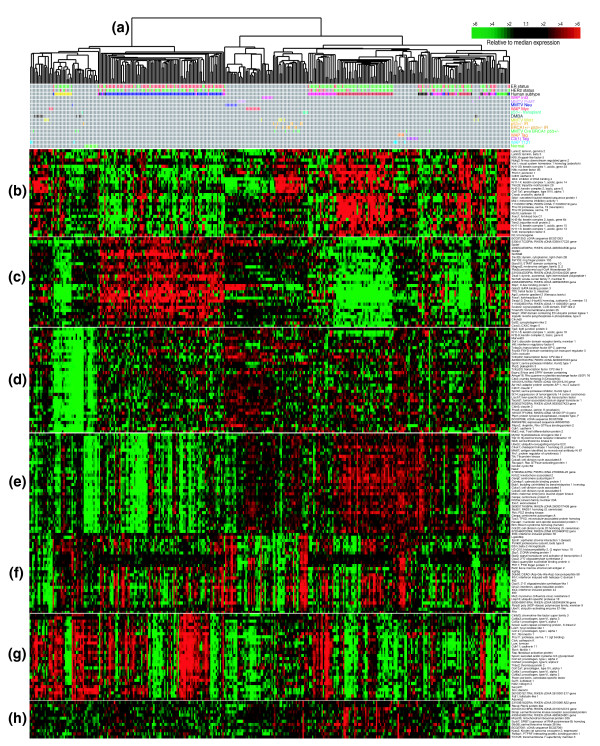
\includegraphics[width=0.8\textwidth]{l6/Gb200785r763}
		\end{column}
	\end{columns}
	\bl{What we learned so far stops working.}
\end{frame}

\begin{frame}{High Dimensional Data}
	\begin{itemize}
		\item We refer to data sets with $p \gg n$ as \e{high dimensional}.
		\item Regression, in particular least squares, is impossible in these cases.
		\item But even if $n > p$ problems can arise.
		\item If $n$ is not much larger than $p$ we are in danger of over-fitting.
		\item At the very least we have to think carefully about the bias-variance trade-off.
		\item Supervised learning on high dimensional data is tricky.
	\end{itemize}
	\bl{We can resort to unsupervised learning, but there also other ways.}
\end{frame}

\begin{frame}{What Goes Wrong in High Dimensions?}
	\begin{center}
		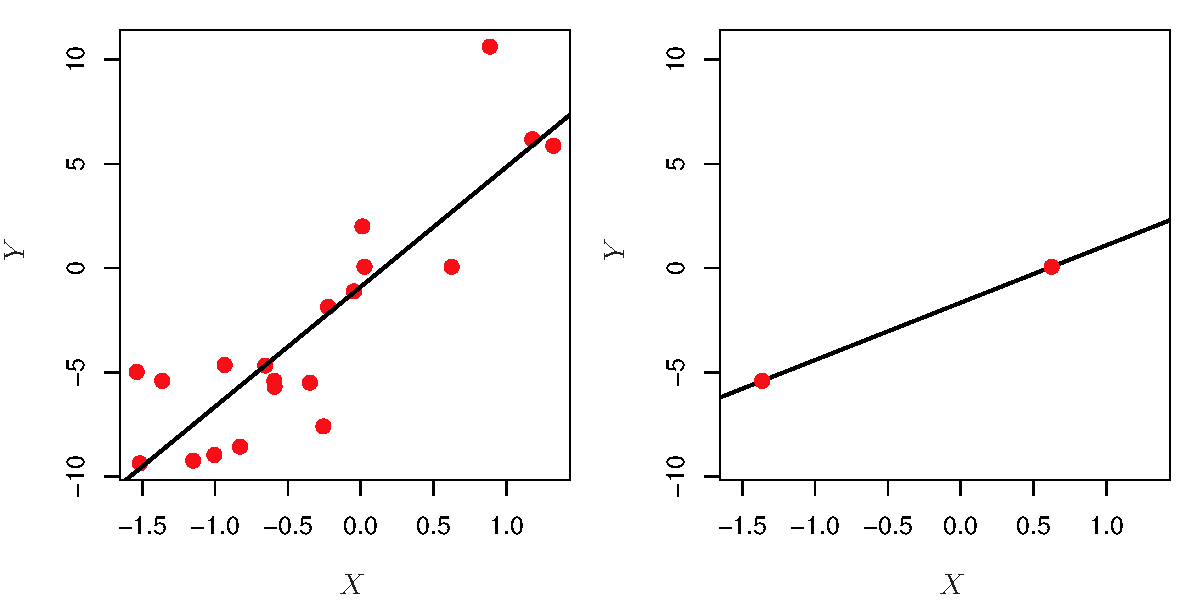
\includegraphics[width=0.8\textwidth]{6_22}
	\end{center}
	\bl{In high dimensions even simple models can be too flexible.}
\end{frame}

\begin{frame}{What Goes Wrong in High Dimensions?}
	\begin{center}
		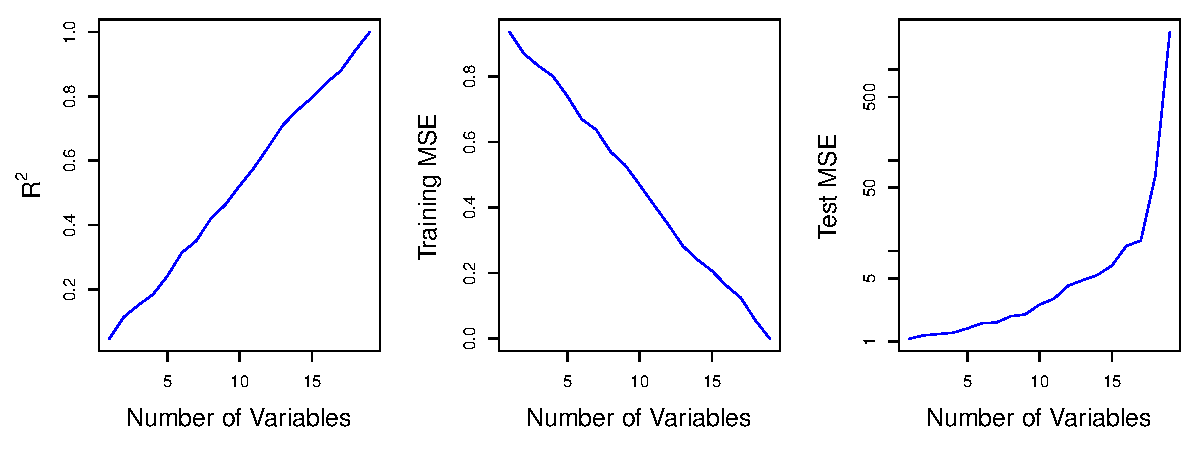
\includegraphics[width=0.9\textwidth]{6_23}
	\end{center}
	\bl{Statistics, like $\bm{R^2}$, can be misleading when predictors are not related to the response.}
\end{frame}

\begin{frame}{Interpretations in High Dimensions}
	\begin{itemize}
		\item We have to very careful when drawing conclusions from high dimensional
			data sets.
		\item For example, suppose we want to find SNPs in an individuals DNA that \\
			are correlated with certain phenotypic traits.
		\item The traits could be affinities to certain diseases. 
		\item Now let's say we find 17 SNPs out of 500,000 that seem to be related to
			high blood pressure.
		\item We should be very careful with the interpretation of this finding.
		\item It is \e{very likely} that we just found \e{one of many} models that suggests a correlation.
		\item That is, there might be a large number of subsets of similar size that wrok equally well.
	\end{itemize}
	\bl{This is by no means an artificial example!}
\end{frame}

\begin{frame}{Dimension Reduction: Feature Selection}
	\begin{itemize}
		\item We can try to reduce the dimensionality by excluding features.
			\begin{cpage}
				\begin{enumerate}
					\item \e{\orange Forward Selection}: start with only the intercept and add
						predictors with the lowest RSS. Proceed until some cutoff is reached. 
					\item \e{\orange Backward Selection}: Start with all variables and keep removing
						the ones with the largest $p$-values. Stop when a cutoff is reached.
					\item \e{\orange Mixed Selection}: Like forward selection, but remove variables
						that acquire large $p$-values after another variable is added.
				\end{enumerate}
			\end{cpage}
		\item This is computationally expensive and of limited use for very high
			dimensions ($p \gg n$).
	\end{itemize}
	\bl{We have seen this before and won't elaborate further on this.}
\end{frame}

\begin{frame}{Dimension Reduction: Principal Components}
	\begin{itemize}
		\item The idea of \e{principal component analysis} (PCA) is to find
			\e{linear combinations} of \\
			predictors that captures the relevant information present in the features. 
		\item PCA allows us to directly quantify which linear combinations are most useful
			for prediction.
		\item Let $Z_1, Z_2, \dots, Z_M$ represent $M < p$ linear combinations of the 
			$p$ predictors:
			\[
				Z_m = \sum_{j=1}^p \phi_{mj} X_j
			\]
			where $ m = 1, 2, \dots, M$.
		\item Unsurprisingly, this is nothing but the matrix multiplication 
			$\bm{Z} = \bm{\phi X}$.
	\end{itemize}
	\bl{Note that the responses are \e{not} used. Therefore PCA is an unsupervised approach.}
\end{frame}

\begin{frame}{Dimension Reduction: Principal Components}
	\begin{itemize}
		\item PCA finds the directions in the feature space along which the \e{observations
			vary the most}.
		\item We can then pick the $M$ combinations (directions) with the highest variance
			and train (fit) our model using $Z_1, \dots, Z_M$ instead of the 
			original $p$ predictors.
		\item That way, we have \e{reduced the dimension} from $p$ to $M$.
		\item Note that we do \e{not} make any assumption what kind of model we are
			going to train.
	\end{itemize}
	\bl{The question is how do we identify these directions.}
\end{frame}

\begin{frame}{Dimension Reduction: Principal Components}
	\vspace{-8mm}
	\begin{center}
		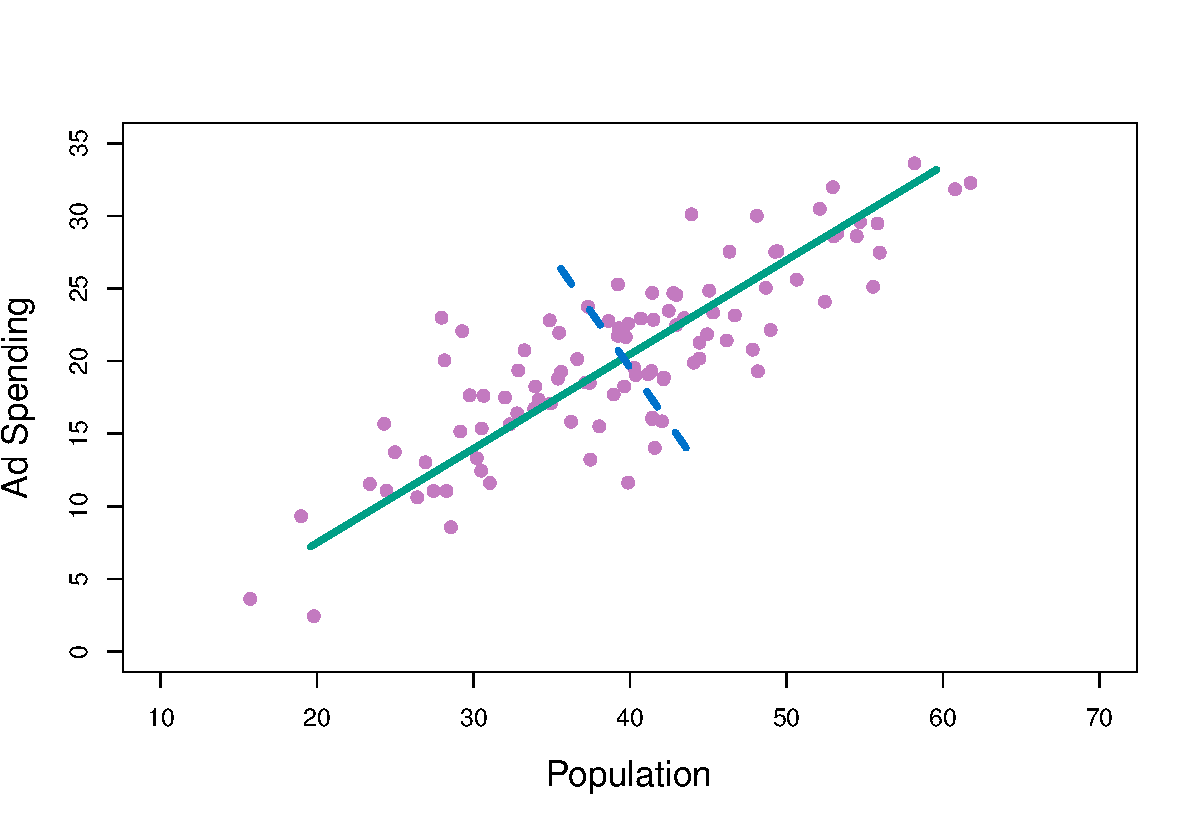
\includegraphics[width=0.6\textwidth]{6_14}
	\end{center}
	\vspace{-6mm}
	\begin{itemize}
		\item The green solid line indicates the \e{first principal component}.
		\item The blue dashed line indicates the \e{second principal component}.
	\end{itemize}
	\bl{The book is a bit shy on the math. We will tell you what really happens.}
\end{frame}

\begin{frame}{Dimension Reduction: Principal Components}
	\vspace{-8mm}
	\begin{center}
		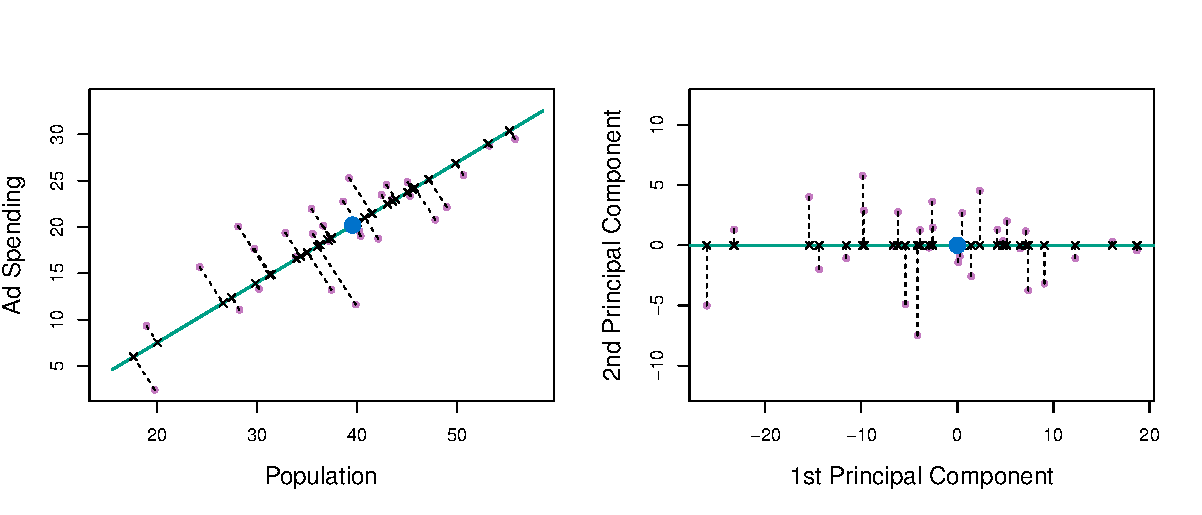
\includegraphics[width=0.9\textwidth]{6_15}
	\end{center}
	\vspace{-6mm}
	\begin{itemize}
		\item Left: before the linear transformation.
		\item Right: after the linear transformation.
	\end{itemize}
	\bl{This is nothing but a rotation in feature space!}
\end{frame}

\begin{frame}{Diagonalising Matrices}
	\begin{itemize}
		\item If a matrix $\bm{A} \in \R^{n\times n}$ can be diagonalised we have:
			\[
				\bm{P}^{-1}\bm{A P} =
				\begin{pmatrix}
					\lambda_1 & 0 & \dots & 0 \\ 
					0 & \lambda_2 & \dots & 0 \\ 
					\vdots & \vdots & \ddots & \vdots \\
					0 & 0 & \dots & \lambda_n \\ 
				\end{pmatrix}
				\implies
				\bm{A P} = \bm{P}
				\begin{pmatrix}
					\lambda_1 & 0 & \dots & 0 \\ 
					0 & \lambda_2 & \dots & 0 \\ 
					\vdots & \vdots & \ddots & \vdots \\
					0 & 0 & \dots & \lambda_n \\ 
				\end{pmatrix}
			\]
			where
			\[ \bm{P} = (\bm{\alpha}_1, \bm{\alpha}_2, \dots, \bm{\alpha}_n) \]
			and
			\[ \bm{A}\bm{\alpha}_i = \lambda_i \bm{\alpha}_i \]
		\item The $\bm{\alpha}_i$ are the \e{normalised eigenvectors} and the $\lambda_i$ the 
			\e{eigenvalues} of $\bm{A}$.
	\end{itemize}
	\bl{In PCA we \e{diagonalise the covariance matrix} and pick components with large $\bm{|\lambda|}$.} 
\end{frame}

\begin{frame}{Principal Component Regression}
	\begin{itemize}
		\item In \e{principal component regression} (PCR) we perform a
			PCA and pick $M < p$ components.
		\item The we perform a linear least square fit on the $Z_1, Z_2, \dots, Z_M$
			instead of the $X_1, X_2, \dots, X_P$.
		\item That is, we fit the model
			\[
				y_i = \theta_0 +
				\sum_{m=1}^M \theta_m z_{im} + \epsilon_i,
				\;\;\; i = 1, 2, \dots, n
			\]
			with
			\[
				\beta_j = \sum_{m=1}^M \phi_{jm} \theta_m
			\]
		\item The $Z_m$ are linear combinations of \e{all} $X_j$.
	\end{itemize}
	\bl{Note that PCR does \e{not} do any feature selection.}
\end{frame}

\begin{frame}{Principal Component Regression}
	\begin{columns}
		\begin{column}{0.6\textwidth}
			\begin{itemize}
				\item We want the model with minimal test MSE.
				\item In practice, we choose $M$ using
					cross-validation.
				\item The more components we include, the more
					flexible the model becomes.
				\item That is, the bias goes down and the
					variance increases.
			\end{itemize}
		\end{column}
		\begin{column}{0.4\textwidth}
			\begin{center}
				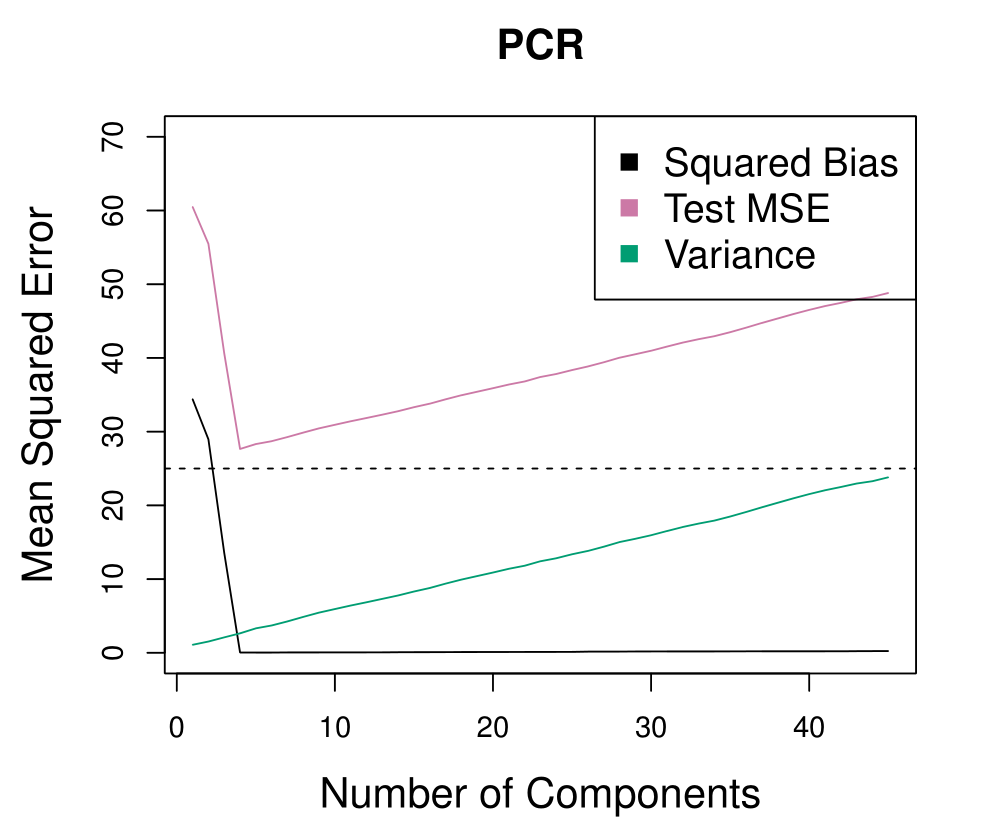
\includegraphics[width=0.95\textwidth]{6_19_l}
			\end{center}
		\end{column}
	\end{columns}
	\bl{This is an artificial data set designed for illustration.}
\end{frame}

\begin{frame}{Partial Least Squares}
	\begin{itemize}
		\item PCA is \e{unsupervised}, it does not take the responses into account.
		\item There is no guarantee that the components that best explain the predictors\\
			are ideal for predicting the response.
		\item \e{Partial least squares} (PLS) tries to address this by taking the response
			into account.
		\item The basic idea is still to find $M < p$ linear combinations
			\[
				Z_m = \sum_{j=1}^p \phi_{mj} X_j
			\]
			in order to reduce the dimensions.
	\end{itemize}
	\bl{PLS is a supervised reduction method.}
\end{frame}

\begin{frame}{Partial Least Squares}
	\begin{itemize}
		\item The computation of the PLS direction proceeds as follows.
			\begin{cpage}
				\begin{enumerate}
					\item \e{\orange First direction, $Z_1$}: we fit  $p$ OLS models
						\[ 
						y_{ji} = \beta_{j0} + \beta_{j1} x_{ji} + \epsilon_i,
						\;\;\; j = 1, 2, \dots, p
						\]
					and then set $\phi_{j1} = \beta_{j1}$:
					\[ Z_1 = \sum_{j=1}^p \phi_{j1} X_j \]
					\item  \e{\orange Rotation}: we rotate all the data in the direction $Z_1$.
					\item  \e{\orange Iteration}: repeat the procedure to obtain $Z_2, \dots, Z_M$.
				\end{enumerate}
			\end{cpage}
	\end{itemize}
	\bl{Just like with PCR, we decide on $\bm{M}$ using cross-validation.}
\end{frame}

\begin{frame}{PCR versus PLS}
	\vspace{-10mm}
	\begin{center}
		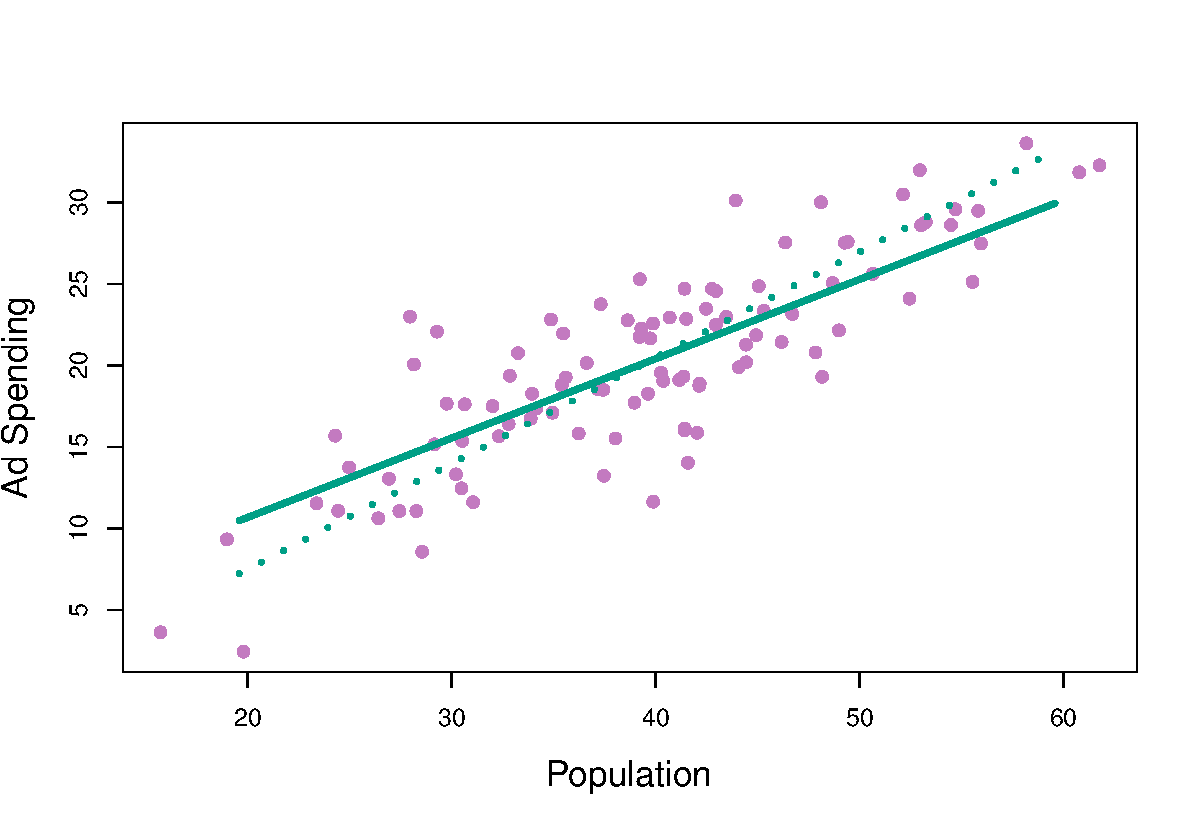
\includegraphics[width=0.7\textwidth]{6_21}
	\end{center}
	\bl{In practice, PLS rarely provides significant benefits over PCR.}
\end{frame}
\end{document}
